\section{Market Microstructure}

Market microstructure is the study of the trading mechanics that are in place 
in real markets. It describes why trading occurs, the rules of trading 
and the protocols to form trades. \citep[p. 3-4]{Has07}
Understanding market microstructure is crucial in designing an artificial market
as without realistic trading setup the representativeness of the model may end
up to be poor and have limited practicality. The goal of an artificial market often
is to recreate phenomena observed in real markets thus the link to the real world 
should be maintained. In this section, the auction theory is briefly introduced and 
then relevant distinctions among market microstructures are discussed. 
Lastly, the common price phenomena, called stylized facts, are presented. Stylized facts
are often used in validating the artificial models. As the literature on decentralized 
markets, as what over-the-counter (OTC) trading is about, is scarce the focus of this thesis is 
on centralized markets. Centralized markets have an exchange in which the trading takes place 
whereas in decentralized markets the buyers and the sellers seek out each other.

% TODO: Maybe extend with behavioural aspects?

\subsection{Double Auction}
% Call market (Itayose, Sealed-bid) vs CDA (Zaraba)

The theoretical foundation of the microstructure in financial markets lies in double auctions.
Double auction market is a special type of auction in which there
are multiple buyers and sellers which both can 
produce quotes and are treated symmetrically \citep*{Kle99}. Buyers
make offers to buy, bid, the traded asset while sellers make offers
to sell, ask, the traded asset \citep*{Moc15}. There are some variations 
between double auction markets. They generally differ in when the order matching 
process takes place and how the orders are matched. 
%In some implementations, such as 
%\citet*{God93}'s, a trade is formed only when a buyer and a seller 
%each agree on the exact trade price but typically the matching of crossing orders is automated.

% \subsubsection{Order Matching in Double Auction}

Typically, the order matching 
is a continuous process occurring after the arrival of each new order but
in some markets this process takes place after a specified time interval
has passed, for example at the end of a trading day. \citep{boer05}
In auction literature, there are various terms used to describe essentially 
the same mechanics. \citet{boer05} used term 
\textit{continuous session market} for the former and \textit{call market}
for the latter whereas \citet{ASt05} called them \textit{Itayose method}
and \textit{Zaraba method} respectively. \citet{Moc15} used term \textit{continuous 
double auction} (CDA) for the former and \textit{periodic double auction} to describe 
the same mechanics of call markets as which they described is an extension of 
a type of auction called sealed-bid. In sealed-bid auctions, the bid and ask offers
are submitted once and then the order matching is executed once. In this thesis,
the terms \textit{continuous double auction} and \textit{call markets} are chosen to describe
these types of markets as they are the most prevalent in the literature.

In call market, the orders are cumulated for a specified time period and the
market is cleared with a single price whereas in continuous market it is done
whenever there are orders that can be matched, and the price is derived from these
orders. \citep{boer05} 
Many real-world stock markets are formed as a hybrid of call and continuous
double auction markets. The price discovery at the beginning and at the end of a 
trading day is conducted with call market mechanics and the trading during the 
typical trading hours is conducted using a continuous environment. \citep{NasdaqClosing05}
For example, Nasdaq's opening and closing call auctions, called opening and closing crosses,
create the official open and close prices of the market and in between the crosses 
trading takes place in a continuous double auction environment \citep{NasdaqCrosses}.  
% More about Sealed-bid matching (supply-demand) and CDA matching
 
\subsection{Execution Systems}
% Quote-driven vs Order-driven
The execution system of a market determines how the orders are matched.
The execution systems are typically divided into two types:
quote-driven and order-driven execution systems. In a quote-driven market, also known
as intermediate markets, the investors trade with prices provided 
by dealers or intermediaries who are part of the market organization. 
In an order-driven market, also called as limit order market, 
the prices are formed according to the orders submitted by the 
investors themselves and trades are formed in a centralized marketplace 
via automatic order matching or with the help of market makers. 
\citep{Baru17} According to \citet{MALINOVA2013104},
the liquidity and price efficiency are generally higher in order-driven 
markets. They also found out that smaller orders get more favourable prices in 
quote-driven markets due to smaller bid-ask spread 
but larger orders benefit from order-driven markets because of the lower 
execution costs. Quote-driven markets are also less transparent compared
to order-driven markets. Real markets, however, are most often a combination
of the two \citep{boer05} but there has been a trend to move from quote-driven
markets to order-driven markets \citep{MALINOVA2013104}.

As simulating intermediate market participants increases complexity
of the model, artificial markets with realistic quote-driven execution are rare. 
However, some artificial markets, such as \citet{SantaFe99}'s, do have some of 
the elements of quote-driven markets in a sense that the prices are driven by 
the sizes of the orders and not the prices offered by the investors or traders. 
Most of the artificial markets found in the ASM literature are order-driven.
% Challenges of quote-driven (clearing is nontrivial)

\subsection{Price Formation}
% Order book, matching and clearing
% Why we do not go deeper to quote-driven:
Price formation is a direct product of the execution system in place in a market
\citep{boer05}. In order-driven markets, price formation is a direct result of the orders
in the limit order book and the matching algorithm in place whereas in quote-driven markets it
is dependent on how the intermediaries view the current and future 
balance between supply and demand of the traded asset. The equilibrium price of a 
quote-driven market is driven by the sizes of the orders and in order-driven markets
it is also driven by the prices submitted with the orders. \citep{MALINOVA2013104}
As quote-driven markets' price formation is somewhat a black box due to the 
dependency on the views and intentions of the intermediaries, it was not considered
as the execution system for the model built in this thesis. On the other hand, 
the price formation of an order-driven market is dependent only on the orders in the
market and the predefined supply-demand matching algorithm in place thus its price 
formation can be described with a greater level of generalization.

% Limit order book and terms
The limit order book is a core component in the price formation in an order-driven market.
Limit order book stores the active limit orders which are simply orders that include the quantity and 
the limit price stated by the trader. The limit price is the maximum price, in case of a bid, or the minimum
price, in case of an ask, that the order can be cleared with. In other words,
bids (asks) cannot be cleared with a price higher (lower) than the limit price stated 
in the order. There are also other types of orders, such as market and 
stop-loss orders, but these can be seen as derivatives from limit orders: 
for example, a bid (an ask) market order is essentially a limit order 
with an extremely high (low) limit price so that it does get matched 
during the clearing process as long as there are opposing limit orders in the 
order book. \citep{lob13} %TODO Supervisor: Voiko taman esittaa esimerkiksi illustrative diagram muodossa?

% Basics of limit order book, supply and demand etc.
A simple limit order book is presented in ~\ref{tbl:orderbook}. This table shows the
quantity of asset bid and asked per each price level: for example, with a price of 5.00
there are 100 unit bid and 200 unit asked. There are, however, more bids and asks that 
accept this price. Those traders that have bid 5.01 and those that have asked 4.99 would obviously also accept
this price. Therefore, it is more informatic to calculate the cumulative sum of the bids and reverse cumulative sum of 
the asks quantities and come up with total quantities of bids and asks per price level that can be matched.  
This order book with cumulative quantities is visualized in figure ~\ref{fig:lob_visual}. Cumulative bids
are renamed as demand and cumulative asks as supply as these terms are more representative in this context.
As there should not be clearable orders in continuous double auction's order book, except very temporarily, 
this example represents more of the state of a limit order book in a call market. Order book
in a continuous double auction is discussed in a moment.

\begin{table}
\centering
\caption{A simple representation of order book}
\label{tbl:orderbook}
\begin{tabular}{lrr}
\toprule
{} &  Bid quantities &  Ask quantities \\
price &                 &                 \\
\midrule
5.04  &               0 &             600 \\
5.03  &               0 &             500 \\
5.02  &              50 &             600 \\
5.01  &             100 &             200 \\
5.00  &             100 &             200 \\
4.99  &             250 &             150 \\
4.98  &             400 &             150 \\
4.97  &             400 &             100 \\
4.96  &             700 &               0 \\
4.95  &             500 &               0 \\
\bottomrule
\end{tabular}
\end{table}
% table.tex > \mytable
\begin{figure}[H]
    \begin{center}  
        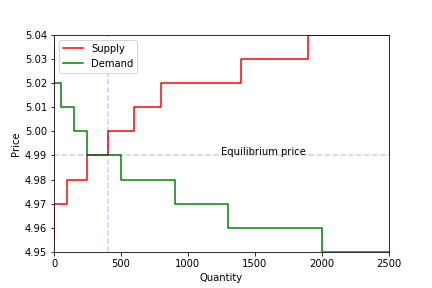
\includegraphics{plots/orderbook_visualized.png}
        \caption{Visualized order book}
        \label{fig:lob_visual}
    \end{center}
\end{figure}

% Price formation in sealed bid/call market
Call markets typically clear at equilibrium price which is the point where
supply and demand cross. To get the equilibrium price, first the maximum clearable quantity
is calculated per price level. This quantity is simply the elementwise
minimum from the supply and the demand arrays. Then the quantity in equilibrium
can be determined by taking the maximum from the maximum clearable quantities
per price level and equilibrium price is simply the price where the maximum clearable quantity
equals the equilibrium quantity. Pseudocode of such an algorithm is illustrated in 
algorithm ~\ref{alg:lob_equil}. After the equilibrium price and quantity have been determined, the 
order matching takes place. The asks are sorted in ascending order using price and bids descending order
and the orders are filled in this order until the sum of filled bids and the sum of filled asks
each equals the equilibrium quantity. It should be noted that not all the bids and the asks with a limit price 
equal to the equilibrium price may be filled, as is the case in the example illustrated in figure ~\ref{fig:lob_visual}. 
Also, it is possible that supply and demand cross in a range of prices meaning that equilibrium price is 
a range of prices. In such a situation it is common to take the mean of these prices and consider that 
as the clearing price.


\begin{algorithm}[H]
    \SetAlgoLined
    \DontPrintSemicolon
    
    bids = sort\_ascending(bids, by price)\;
    asks = sort\_descending(asks, by price)\;
    \;
    demand = cumulative\_sum(bids, using quantity)\;
    supply = cumulative\_sum(asks, using quantity)\;
    \;
    maximum clearable per price = elementwise\_min\_per\_price(demand, supply)\;
    \;
    equilibrium quantity = max(maximum clearable per price)\;
    equilibrium price = price where (maximum clearable per price == equilibrium quantity)\;
    \KwResult{Equilibrium price and quantity}
    \caption{Pseudo algorithm for finding market equilibrium}
    \label{alg:lob_equil}
\end{algorithm}

In a continuous double auction, the matching process is slightly simpler in computation
sense as there is no need to find a common price for many orders. Only the latest arrived
order needs to be cleared with opposing orders or checked whether it can be cleared. A continuous
double auction does not accumulate crossing orders in a similar fashion as call markets do. 
In principle, the same algorithm used in a call market could be used also in a continuous double auction 
but typically the surplus distribution is different. Unlike in call markets where the surplus is often
split among the crossing orders, in a continuous double auction the surplus goes to the trader who made the 
latest order. In other words, the trade prices are drawn from the orders that were already in the limit 
order book. This sort of matching could be conducted by looping and clearing the opposing side of the 
order book until either there are no more crossing orders with the newly arrived order, or the new 
order is already cleared completely. In case of the newly arrived order is not completely cleared after 
depleting all possible crossing orders, the order is inserted to the order book and the clearing process 
ends. If there were no crossing orders, to begin with, the newly arrived is put to the order book immediately. 
This algorithm is illustrated in algorithm ~\ref{alg:lob_cont}. For further reading, an extensive and 
thorough overview of the mechanics of limit order book markets is provided by \citet{lob13}. A detailed 
explanation about the rules of trading and matching engine of Nasdaq Nordic market model from \citet{NasdaqModel}.

\begin{algorithm}[H]
    \SetAlgoLined
    \DontPrintSemicolon
    \uIf{new order is bid}{
        asks = get\_asks(order book)\;
        price of new order = get\_price(new order)\;

        \While{(min\_price(asks) $\geq$ price of new order) \\
        \hskip\algorithmicindent\& (get\_quantity(new order) > 0)}{
            crossing orders = filter(asks, where price $\geq$ get\_price(new order))\;
            opposite order = get\_next(crossing orders)\;
            clear(new order, opposite order)\;
        }
    }
    \uElseIf{new order is ask}{
        bids = get\_bids(order book)\;
        price of new order = get\_price(new order)\;
        
        \While{(min\_price(bids) $\leq$ price of new order) \\ 
        \hskip\algorithmicindent \& (get\_quantity(new order) > 0)}{
            crossing orders = filter(bids, where price $\leq$ get\_price(new order))\;
            opposite order = get\_next(crossing orders)\;
            clear(new order, opposite order)\;
        }
    }
    \uIf{get\_quantity(new order) > 0}{
        insert\_to\_orderbook(new order)\;
    }

    \caption{Pseudo algorithm for clearing continuous double auction}
    \label{alg:lob_cont}
\end{algorithm}


\subsection{Price Dynamics}
% Stylized facts
The price dynamics in stock markets are known to be chaotic and difficult to 
analyze. The underlying elements that play a role in the price dynamics
are constantly evolving and they remain relatively poorly understood.
However, there are some characteristics of price behaviour that are supported
with enough empirical evidence to be considered as properties of price in
financial markets. These statistical phenomena, called stylized facts in
econometrics, have been observed in extensive amount of studies across 
different assets, markets and time periods \citep{Shakeel18}. 
% List of Stylized facts (Cont R. (2001) & Gould et al. (2013))
According to \citet{StylizedFacts01} and \citet{lob13}, price related stylized
facts include:

\begin{enumerate}
    \item Fat-tailed distribution of returns: distribution of asset returns has fatter tails than normal distribution meaning that they have positive excess kurtosis. 
          In the figure  ~\ref{fig:sp_fat_tails} distributions of daily rate of returns of S\&P 500 returns are shown.
    \par
    \begin{minipage}{\linewidth}
        \centering
        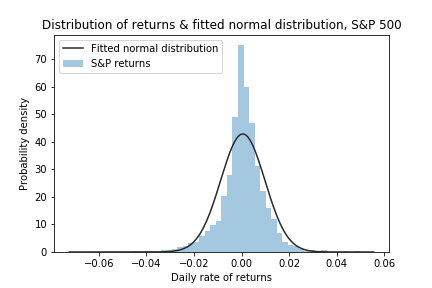
\includegraphics[width=10cm]{plots/S&P500_fat_tails.png}
        \captionof{figure}{Fat-tailed of returns of S\&P 500}
        \label{fig:sp_fat_tails}
    \end{minipage}
    \item Lack of autocorrelation: autocorrelation of returns in financial markets have been shown to be statistically insignificant, except in the very short term. 
          Previous returns have no predictive power over the future returns of a stock. 
          Figure ~\ref{fig:sp_autocorr} illustrates the autocorrelation of daily returns of S\&P 500.
          As seen in the figure, the autocorrelations of all of the lags lie inside the blue area meaning that all of the lags 
          are not statistically significant from zero.
    \par
    \begin{minipage}{\linewidth}
        \centering
        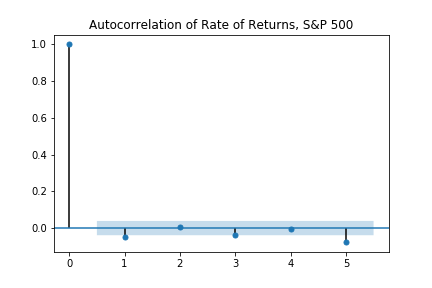
\includegraphics[width=10cm]{plots/S&P500_autocorr.png}
        \captionof{figure}{Absence of autocorrelation in S\&P 500}
        \label{fig:sp_autocorr}
    \end{minipage}
    \item Volatility clusters: volatility has been measured to have positive autocorrelation. 
          Additional exceptional price movements tend to follow big price movements forming clusters of volatility throughout time.
          As can be observed from the figure ~\ref{fig:sp_volaclusters}, there are volatility clusters for up to ten weeks in 
          S\&P 500 as the autocorrelation of volatility is positive up to that point. 
          The figure illustrates the autocorrelation of weekly daily returns in S\&P 500.  
    \par
    \begin{minipage}{\linewidth}
        \centering
        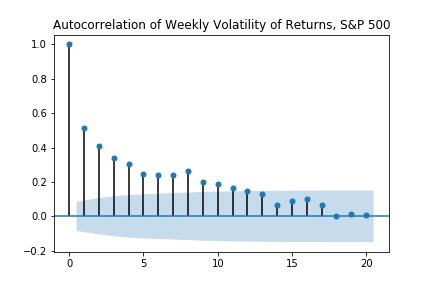
\includegraphics[width=10cm]{plots/S&P500_vola_autocorr.png}
        \captionof{figure}{Volatility clustering in S\&P 500}
        \label{fig:sp_volaclusters}
    \end{minipage}
\end{enumerate} 



% Something about theories of these things (explanation for the stylized facts)
% file:///D:/Opinnot/Master's%20Thesis/literature/real%20markets/price%20dynamics/TheoriesExplainingStockPriceBehavior%20(1).pdf

All of the figures above utilize daily adjusted close prices for S\&P 500 stock index 
for the time range from 1.1.2010 to 1.1.2020. 
As has been done in the literature of artificial markets, the 
representativeness of the ASM model built in this thesis is validated also 
using these stylized facts.